\documentclass[12pt]{article}
\usepackage{amsmath}
\usepackage{graphicx}
\usepackage{hyperref}
\usepackage{listings}
\usepackage{color}

\title{Operating System Course Report - First Half of the Semester}
\author{B class}
\date{\today}

\begin{document}

\maketitle
\newpage

\tableofcontents
\newpage

\section{Introduction}
This report summarizes the topics covered during the first half of the Operating System course. It includes theoretical concepts, practical implementations, and assignments. The course focuses on the fundamentals of operating systems, including system architecture, process management, CPU scheduling, and deadlock handling.

\section{Course Overview}
\subsection{Objectives}
The main objectives of this course are:
\begin{itemize}
    \item To understand the basic components and architecture of a computer system.
    \item To learn process management, scheduling, and inter-process communication.
    \item To explore file systems, input/output management, and virtualization.
    \item To study the prevention and handling of deadlocks in operating systems.
\end{itemize}

\subsection{Course Structure}
The course is divided into two halves. This report focuses on the first half, which covers:
\begin{itemize}
    \item Basic Concepts and Components of Computer Systems
    \item System Performance and Metrics
    \item System Architecture of Computer Systems
    \item Process Description and Control
    \item Scheduling Algorithms
    \item Process Creation and Termination
    \item Introduction to Threads
    \item File Systems
    \item Input and Output Management
    \item Deadlock Introduction and Prevention
    \item User Interface Management
    \item Virtualization in Operating Systems
\end{itemize}

\section{Topics Covered}

\subsection{Basic Concepts and Components of Computer Systems}
This section explains the fundamental components that make up a computer system, including the CPU, memory, storage, and input/output devices.

\subsection{System Performance and Metrics}
This section introduces various system performance metrics used to measure the efficiency of a computer system, including throughput, response time, and utilization.

\subsection{System Architecture of Computer Systems}
Describes the architecture of modern computer systems, focusing on the interaction between hardware and the operating system.

\subsection{Process Description and Control}
Processes are a central concept in operating systems. This section covers:
\begin{itemize}
    \item Process states and state transitions
    \item Process control block (PCB)
    \item Context switching
\end{itemize}

\subsection{Scheduling Algorithms}
This section covers:
\begin{itemize}
    \item First-Come, First-Served (FCFS)
    \item Shortest Job Next (SJN)
    \item Round Robin (RR)
\end{itemize}
It explains how these algorithms are used to allocate CPU time to processes.

\subsection{Process Creation and Termination}
Details how processes are created and terminated by the operating system, including:
\begin{itemize}
    \item Process spawning
    \item Process termination conditions
\end{itemize}

\subsection{Introduction to Threads}
This section introduces the concept of threads and their relation to processes, covering:
\begin{itemize}
    \item Single-threaded vs. multi-threaded processes
    \item Benefits of multithreading
\end{itemize}

\subsection{File Systems}
File systems provide a way for the operating system to store, retrieve, and manage data. This section explains:
\begin{itemize}
    \item File system structure
    \item File access methods
    \item Directory management
\end{itemize}

\subsection{Input and Output Management}
Input and output management is key for handling the interaction between the system and external devices. This section includes:
\begin{itemize}
    \item Device drivers
    \item I/O scheduling
\end{itemize}

\subsection{Deadlock Introduction and Prevention}
Explores the concept of deadlocks and methods for preventing them:
\begin{itemize}
    \item Deadlock conditions
    \item Deadlock prevention techniques
\end{itemize}

\subsection{User Interface Management}
This section discusses the role of the operating system in managing the user interface. Topics covered include:
\begin{itemize}
    \item Graphical User Interface (GUI)
    \item Command-Line Interface (CLI)
    \item Interaction between the user and the operating system
\end{itemize}

\subsection{Virtualization in Operating Systems}
Virtualization allows multiple operating systems to run concurrently on a single physical machine. This section explores:
\subsubsection{Pengertian Virtualisasi Sistem Operasi}
    \par Virtualisasi adalah teknologi yang memungkinkan beberapa sistem operasi (OS) berjalan secara bersamaan pada satu mesin fisik. Ini dicapai dengan membuat lingkungan virtual yang memisahkan perangkat keras dari perangkat lunak. Setiap OS yang berjalan di atas mesin virtual (VM) beroperasi seolah-olah memiliki sumber daya perangkat keras yang berdedikasi, meskipun pada kenyataannya perangkat keras tersebut dibagi oleh beberapa VM.

    \begin{figure}[h!]
    \centering
    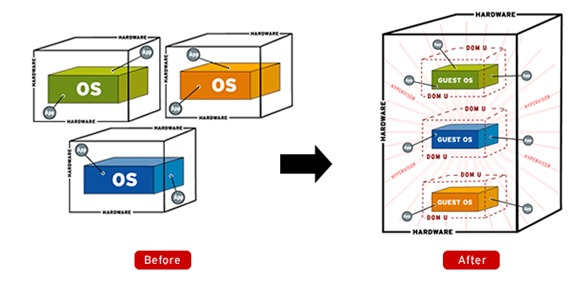
\includegraphics[width=0.8\textwidth]{assets/carakerjavirtualisasi.jpg}
    \caption{Cara Kerja Virtualisasi}
    \label{fig:label_gambar}
\end{figure}
Pada ilustrasi gambar, terlihat dua kondisi:
\begin{itemize}
    \item Sebelum Virtualisasi (Before): Di sisi kiri gambar, kita melihat bahwa setiap sistem operasi (OS) berjalan langsung di atas perangkat keras yang terpisah. Pendekatan ini kurang efisien karena setiap OS membutuhkan perangkat kerasnya sendiri, yang menyebabkan pemborosan sumber daya fisik ketika perangkat keras tidak dimanfaatkan secara maksimal.
    \item Setelah Virtualisasi (After): Di sisi kanan gambar, terlihat bahwa setelah virtualisasi diterapkan, satu perangkat keras fisik dapat menjalankan beberapa OS sekaligus melalui penggunaan hypervisor. Hypervisor ini menciptakan beberapa mesin virtual (VM) yang memungkinkan berbagai sistem operasi berjalan di atas satu perangkat keras secara bersamaan. Hal ini meningkatkan efisiensi penggunaan sumber daya dan fleksibilitas dalam pengelolaan sistem.
\end{itemize}

Dengan cara ini, virtualisasi memungkinkan pemanfaatan sumber daya yang lebih baik, meningkatkan isolasi antar sistem, dan mempermudah proses pemeliharaan serta pengelolaan infrastruktur komputasi.


\subsubsection{Jenis Jenis Virtualisasi pada Sistem Operasi}
\subsubsection{Komponen Virtualisasi Sistem Operasi}
\subsubsection{Hypervisor dan Virtual Machines}
\subsubsection{Contoh Penerapan Virtualisasi pada Sistem Operasi}
\subsubsection{Keuntungan dan Kerugian Virtualisasi}

\begin{enumerate}
    \item \textbf{Keuntungan dari Virtualisasi}
    \par Virtualisasi menawarkan banyak keuntungan baik secara operasional maupun finansial, yang membuatnya menjadi kunci dalam komputasi enterprise dan pengembangan perangkat lunak. Berikut ini adalah beberapa keuntungan utama dari virtualisasi: 

\begin{itemize}
    \item \textbf{Menggunakan Perangkat Keras yang Ada dengan Lebih Baik:} 
    Prosesor modern berkembang dengan cepat, dari 8-bit hingga 64-bit, serta jumlah inti prosesor yang terus bertambah. Dengan menjalankan beberapa mesin virtual pada satu server fisik, pengguna dapat mengoptimalkan penggunaan perangkat keras yang ada. Sistem multi-core dapat menjalankan beberapa mesin virtual di setiap inti prosesor yang berbeda, memaksimalkan efisiensi sumber daya.
    
    \item \textbf{Mengurangi Harga Perangkat Keras:} 
    Virtualisasi memungkinkan pengguna untuk menambah server atau layanan tanpa harus membeli perangkat keras baru, yang pada akhirnya mengurangi biaya secara signifikan.
    
    \item \textbf{Mengurangi Infrastruktur IT:} 
    Server fisik membutuhkan listrik, ruang, dan pendinginan. Dengan virtualisasi, kebutuhan akan listrik, ruang, dan pendinginan bisa dikurangi karena satu server fisik dapat menjalankan banyak mesin virtual.
    
    \item \textbf{Menyederhanakan Administrasi Sistem:} 
    Dengan menjalankan beberapa mesin virtual pada satu perangkat keras fisik, kesehatan sistem bisa lebih mudah dipantau, dan administrasi sistem dapat disederhanakan, terutama dalam hal migrasi atau cloning ketika terjadi kesalahan perangkat keras.
    
    \item \textbf{Meningkatkan Uptime dan Mempercepat Failure Recovery:} 
    Portabilitas mesin virtual memudahkan pemindahan dari satu server fisik ke server lain jika ada masalah pada perangkat keras, tanpa mengganggu operasi yang sedang berjalan.
    
    \item \textbf{Menyederhanakan Ekspansi Kapasitas:} 
    Mesin virtual dapat dipindahkan dengan mudah ke perangkat keras baru dengan spesifikasi yang lebih tinggi, seperti prosesor yang lebih cepat, memori yang lebih besar, atau kapasitas jaringan yang lebih tinggi.
    
    \item \textbf{Dukungan Perangkat Lunak Asli yang Lebih Mudah:} 
    Dengan virtualisasi, pengguna dapat menjalankan sistem operasi lama di partisi logis, sehingga memungkinkan perangkat lunak lama tetap berjalan meskipun sistem operasi sudah diperbarui.
    
    \item \textbf{Menyederhanakan Pengembangan dan Testing Aplikasi:} 
    Pengembangan dan pengujian aplikasi pada berbagai sistem operasi menjadi lebih mudah dengan virtualisasi, karena mesin virtual dapat menjalankan berbagai sistem operasi tanpa perlu perangkat keras khusus.
\end{itemize}


    \item \textbf{Kerugian Virtualisasi}
    \par Walaupun virtualisasi menawarkan banyak keuntungan, ada beberapa kerugian yang perlu diperhatikan, di antaranya:

\begin{itemize}
    \item \textbf{Satu Titik Kesalahan:} 
    Jika satu perangkat keras fisik digunakan untuk menjalankan banyak server virtual, kerusakan pada perangkat keras tersebut bisa memengaruhi semua server virtual yang berjalan di atasnya. Oleh karena itu, diperlukan strategi cadangan dan monitoring untuk meminimalkan risiko ini.
    
    \item \textbf{Kepadatan Saluran Jaringan:} 
    Jika satu server fisik menjalankan banyak mesin virtual yang membutuhkan akses jaringan intensif, ini bisa menyebabkan kepadatan saluran jaringan dan menurunkan kinerja jaringan. Solusi untuk masalah ini adalah dengan menggunakan beberapa kartu jaringan pada host fisik.
    
    \item \textbf{Meningkatkan Kompleksitas Jaringan dan Debugging:} 
    Virtualisasi jaringan yang kompleks dapat menambah kesulitan dalam hal desain dan pengelolaan infrastruktur, serta memakan lebih banyak waktu dalam proses debugging.
    
    \item \textbf{Meningkatkan Kompleksitas Administrasi:} 
    Administrasi bisa menjadi lebih rumit jika sistem manajemen terdistribusi yang digunakan tidak mendukung mesin virtual. Oleh karena itu, diperlukan perencanaan dan pemilihan alat yang tepat untuk mendukung virtualisasi secara efisien.
\end{itemize}
\end{enumerate}

\subsubsection{Kesimpulan}
Virtualisasi merupakan teknologi penting dalam komputasi modern, yang memungkinkan pemanfaatan sumber daya secara lebih efisien, meningkatkan fleksibilitas, dan menyederhanakan pengelolaan infrastruktur. Meskipun memiliki beberapa kelemahan seperti potensi satu titik kesalahan dan peningkatan kompleksitas jaringan, manfaat yang diperoleh jauh lebih besar, terutama dalam hal penghematan biaya dan peningkatan uptime sistem.

\newpage

\begin{thebibliography}{9}
    \bibitem{Ref1} Tanenbaum, A. S., \& Bos, H. (2015). \textit{Modern Operating Systems}. Pearson.
    
    \bibitem{Ref2} Silberschatz, A., Galvin, P. B., \& Gagne, G. (2018). \textit{Operating System Concepts}. John Wiley \& Sons.
    
    \bibitem{Ref3} Singh, G. (2019). \textit{Virtualization Essentials}. John Wiley \& Sons.
    
    \bibitem{Ref4} Barham, P., Dragovic, B., Fraser, K., Hand, S., Harris, T., Ho, A., \& Warfield, A. (2003). \textit{Xen and the art of virtualization}. In \textit{Proceedings of the nineteenth ACM symposium on Operating systems principles} (pp. 164-177).
\end{thebibliography}


\section{Assignments and Practical Work}
\subsection{Assignment 1: Process Scheduling}
Students were tasked with implementing various process scheduling algorithms (e.g., FCFS, SJN, and RR) and comparing their performance under different conditions.

\subsection{Assignment 2: Deadlock Handling}
In this assignment, students were asked to simulate different deadlock scenarios and explore various prevention methods.

\subsection{Assignment 3: Multithreading and Amdahl's Law}
This assignment involved designing a multithreading scenario to solve a computationally intensive problem. Students then applied *Amdahl's Law* to calculate the theoretical speedup of the program as the number of threads increased.

\textbf{Tujuan:}  
Mendesain skenario multithreading untuk menyelesaikan masalah komputasi intensif dan menerapkan *Hukum Amdahl* untuk menghitung percepatan teoretis.

\textbf{Pernyataan Masalah:}  
Misalkan sebuah program memiliki 70\% waktu eksekusi yang dapat diparalelkan. Tujuannya adalah menemukan percepatan teoretis ketika menggunakan 4 thread, berdasarkan *Hukum Amdahl*.

\textbf{Penyelesaian:}  
*Hukum Amdahl* digunakan untuk menghitung percepatan teoretis dari suatu program ketika sebagian dari program tersebut dapat diparalelkan. *Hukum Amdahl* dinyatakan sebagai:

\[
S(N) = \frac{1}{(1 - P) + \frac{P}{N}}
\]

dimana:
\begin{itemize}
    \item \( S(N) \) adalah percepatan dengan \( N \) thread.
    \item \( P \) adalah fraksi dari program yang dapat diparalelkan.
    \item \( N \) adalah jumlah thread.
\end{itemize}

Untuk tugas ini:
\[
P = 0.7 \quad \text{(70\% dari program dapat diparalelkan)}
\]
\[
N = 4 \quad \text{(4 thread)}
\]

Substitusikan nilai ke dalam *Hukum Amdahl*:
\[
S(4) = \frac{1}{(1 - 0.7) + \frac{0.7}{4}}
\]
\[
S(4) = \frac{1}{0.3 + 0.175} = \frac{1}{0.475} \approx 2.11
\]

Dengan demikian, percepatan teoretis menggunakan 4 thread adalah sekitar \( 2.11 \).

\textbf{Kesimpulan:}  
Menggunakan 4 thread menghasilkan percepatan sekitar 2.11 kali untuk sebuah program yang 70\% eksekusinya dapat diparalelkan. Hal ini menunjukkan bahwa meskipun multithreading meningkatkan kinerja, percepatan dibatasi oleh bagian dari program yang tidak dapat diparalelkan, seperti yang dijelaskan oleh *Hukum Amdahl*.


\subsection{Assignment 4: Simple Command-Line Interface (CLI) for User Interface Management}
Students were tasked with creating a simple *CLI* for user interface management. The CLI should support basic commands such as file manipulation (creating, listing, and deleting files), process management, and system status reporting.

\textbf{Tujuan:}  
Membuat antarmuka baris perintah (*Command-Line Interface*, CLI) sederhana yang mendukung manipulasi file dasar, manajemen proses, dan pelaporan status sistem.

\textbf{Pernyataan Masalah:}  
CLI harus mendukung perintah-perintah berikut:
\begin{itemize}
    \item \texttt{buat\_file <nama\_file>} - Membuat file baru dengan nama yang ditentukan.
    \item \texttt{hapus\_file <nama\_file>} - Menghapus file yang ditentukan.
    \item \texttt{daftar\_file} - Menampilkan semua file di direktori saat ini.
    \item \texttt{jalankan\_proses <nama\_proses>} - Menjalankan proses yang ditentukan.
    \item \texttt{matikan\_proses <id\_proses>} - Menghentikan proses dengan ID yang ditentukan.
    \item \texttt{status\_sistem} - Menampilkan penggunaan CPU, memori, dan proses yang sedang berjalan.
\end{itemize}

\textbf{Penyelesaian:}  
Berikut adalah contoh implementasi CLI:

\begin{lstlisting}[language=bash, caption=Contoh skrip CLI sederhana]
#!/bin/bash

function buat_file() {
    touch $1
    echo "File '$1' dibuat."
}

function hapus_file() {
    rm $1
    echo "File '$1' dihapus."
}

function daftar_file() {
    ls
}

function jalankan_proses() {
    $1 &
    echo "Proses '$1' dimulai dengan PID $!"
}

function matikan_proses() {
    kill $1
    echo "Proses dengan PID $1 dihentikan."
}

function status_sistem() {
    echo "Penggunaan CPU: $(top -bn1 | grep "Cpu(s)" | awk '{print $2 + $4}')%"
    echo "Penggunaan Memori: $(free -m | awk 'NR==2{printf "%.2f", $3*100/$2 }')%"
    echo "Proses yang Berjalan:"
    ps
}

# Interpretasi perintah CLI
case "$1" in
    buat_file) buat_file $2 ;;
    hapus_file) hapus_file $2 ;;
    daftar_file) daftar_file ;;
    jalankan_proses) jalankan_proses $2 ;;
    matikan_proses) matikan_proses $2 ;;
    status_sistem) status_sistem ;;
    *) echo "Perintah tidak valid." ;;
esac
\end{lstlisting}

\textbf{Kesimpulan:}  
Skrip di atas menyediakan antarmuka baris perintah sederhana untuk manajemen file, proses, dan status sistem. Skrip ini mendemonstrasikan manipulasi file dasar, kontrol proses, dan pemantauan sistem secara real-time, memenuhi persyaratan tugas.

\begin{thebibliography}{9}

\bibitem{Amdahl1967} 
Amdahl, G. M. (1967). 
\textit{Validity of the Single Processor Approach to Achieving Large Scale Computing Capabilities}. 
AFIPS Spring Joint Computer Conference, 30, 483-485.

\bibitem{LinuxCommandLine} 
Negus, C. (2019). 
\textit{Linux Command Line and Shell Scripting Bible}. 
Wiley.

\end{thebibliography}

\subsection{Assignment 5: File System Access}
In this assignment, students implemented file system access routines, including:
\begin{itemize}
    \item File creation and deletion
    \item Reading from and writing to files
    \item Navigating directories and managing file permissions
\end{itemize}

\section{Conclusion}
The first half of the course introduced core operating system concepts, including process management, scheduling, multithreading, and file system access. These topics provided a foundation for more advanced topics to be covered in the second half of the course.

\end{document}